\documentclass{bcrre_exam}


\title{Designing Track Alignment Worksheet}
\author{}
\date{May 2025}

\printanswers

\begin{document}

\maketitle

\section*{Aim}
In this workshop session you are going to work through some of the equations and calculations you were introduced to in the preparatory videos. You will then go on to look at how to design a horizontal and a vertical curve.

\section*{Learning Outcomes}

\begin{itemize}
    \item To become familiar in some frequently used calculations
    \item To improve confidence in using these calculations
\end{itemize}

\newpage
\section{Calculating Cant}

There are 3 measures related to cant, $E_q$ equilibrium cant, $E_a$ applied cant, and, $D$ cant deficiency. All are measured in \unit{mm}.

As shown in equation \ref{eq:eq_ea_d}, equilibrium cant is always equal to the sum of applied cant and cant deficiency.

\begin{equation}
    \label{eq:eq_ea_d}
    E_q = E_a+D
\end{equation}

The equations in \ref{eq:e_rot} gives an approximation for calculating applied cant and cant deficiency that shall be used in this worksheet. The applied cant will be two thirds of the calculated equilibrium cant and therefore one third of the calculated equilibrium cant will be cant deficiency.

\begin{equation}
    \label{eq:e_rot}
        E_a = \frac{2}{3}E_q\ , \quad
        D = \frac{E_a}{2}
\end{equation}

Equation \ref{eq:eq_calc} gives the calculation for equilibrium cant.

\begin{equation}
    \label{eq:eq_calc}
    E_q=\frac{11.82 V^2}{R}
\end{equation}

Where:
\begin{itemize}
    \item $E_q$: equilibrium cant (\unit{mm})
    \item $V$: velocity (\unit{km/h})
    \item $R$: curve radius (\unit{m})
\end{itemize}


\begin{questions}

\question
What is the equilibrium cant for a track for a curve with a rolling stock speed of \qty{85}{km/h} and a radius of \qty{500}{m}?

\begin{solution}
    $E_q=$ \qty{170.8}{mm}
    
    \begin{equation}
        E_q=\frac{11.82 \cdot 85^2}{500} = 170.8
    \end{equation}
\end{solution}

\question
What is the equilibrium cant for a track for a curve with a rolling stock speed of \qty{56}{km/h} and a radius of \qty{300}{m}?

\begin{solution}
    $E_q=$ \qty{123.6}{mm}
    
    \begin{equation}
        E_q=\frac{11.82 \cdot 56^2}{300} = 123.6
    \end{equation}
\end{solution}

\question
What is the equilibrium cant for a track for a curve with a rolling stock speed of \qty{120}{km/h} and a radius of \qty{800}{m}?

\begin{solution}
    $E_q=$ \qty{212.8}{mm}
    
    \begin{equation}
        E_q=\frac{11.82 \cdot 120^2}{800} = 212.8
    \end{equation}
\end{solution}

\question
Using equation \ref{eq:e_rot} and a maximum allowed cant $E_{a(max)}$ of \qty{150}{mm}:
\begin{itemize}
    \item What would the applied cant, $E_a$ be in each of the previous questions?
    \item In which cases would a speed limit need to be applied?
\end{itemize}

\begin{solution}
    
    
    \textbf{Question 1:} 
    
    $V=$ \qty{85}{km/h} and $R=$ \qty{500}{m}

    $E_a=170.8 \cdot \frac{2}{3}=$ \qty{133.9}{mm}

    No speed limit needed.

    \textbf{Question 2:} 
    
    $V=$ \qty{56}{km/h} and $R=$ \qty{300}{m}

    $E_a=123.6 \cdot \frac{2}{3}=$ \qty{82.4}{mm}

    No speed limit needed.

    \textbf{Question 3:} 
    
    $V=$ \qty{120}{km/h} and $R=$ \qty{800}{m}

    $E_a=212.8 \cdot \frac{2}{3}=$ \qty{141.8}{mm}

    No speed limit needed.
    
\end{solution}

\end{questions}

\newpage
\section{Designing an Alignment}

Rearranging equation \ref{eq:eq_calc}, it is possible to calculate the radius of a curve and the maximum velocity.

\begin{questions}

\question
For all questions in this section assume that the maximum applied cant for a curve is \qty{150}{mm}.

Using equation \ref{eq:e_rot}, if a curve uses the maximum applied cant, what is the equilibrium cant $E_q$?

\begin{solution}
    $E_q=$ \qty{225}{mm}
    \begin{equation}
        E_q = \frac{3}{2} \cdot E_a = \frac{3}{2} \cdot 150 = 225
    \end{equation}
\end{solution}
\vspace{1cm}
{\Large \bfseries Radius}

\question
You are designing a curve for a new alignment. The track speed will be \qty{180}{km/h} and a maximum applied cant will be used. 

What should the radius of this curve be?

\begin{solution}
    $R=$ \qty{1702}{m}
    
    \begin{equation}
        R=\frac{11.82 \cdot V^2}{E_q}=\frac{11.82 \cdot 180^2}{225}=1702
    \end{equation}
\end{solution}

\question
The designer of a new track would like to cut costs by reducing the radius of a curve on a \qty{270}{km/h} railway alignment to \qty{3000}{m}.

What is your advice?

\begin{solution}
    $R=$ \qty{3830}{m}
    
    \begin{equation}
        R=\frac{11.82 \cdot V^2}{E_q}=\frac{11.82 \cdot 270^2}{225}=3830
    \end{equation}

    As the radius of the curve should be \qty{3830}{m}, reducing it may be unadvisable as it may increase the risk of derailment. You could argue about the use of tilting trains or a risk assessment needing to be written.
\end{solution}
\vspace{1cm}
{\Large \bfseries Velocity}

\question
What is the maximum speed on a corner of \qty{750}{m} with the maximum applied cant?

\begin{solution}
    $V=$ \qty{119}{km/h}
    
    \begin{equation}
        V=\sqrt{\frac{E_q \cdot R}{11.82}}=\sqrt{\frac{225 \cdot 750}{11.82}}=119
    \end{equation}
\end{solution}

\question
How would this speed change if the applied cant were reduced to \qty{110}{mm}?

\begin{solution}
    $V=$ \qty{102}{km/h}

    \begin{equation}
        E_q = \frac{3}{2} \cdot E_a = \frac{3}{2} \cdot 110 = 165
    \end{equation}
    
    \begin{equation}
        V=\sqrt{\frac{E_q \cdot R}{11.82}}=\sqrt{\frac{165 \cdot 750}{11.82}}=102
    \end{equation}
\end{solution}

\end{questions}

\newpage
\section{Jerk} 

The physical property of excessive jerk is what we want to avoid, as it makes a journey uncomfortable for passengers. Some limits for jerk include:

Lateral jerk limit: \qty{0.2}{\meter \per \second \cubed}

Longitudinal jerk (comfortable limit): \qty{0.3}{\meter \per \second \cubed}

Longitudinal jerk (extreme limit): \qty{0.5}{\meter \per \second \cubed}

jerk is the third derivative of displacement, equations \ref{eq:vel}, \ref{eq:acc}, and, \ref{eq:jerk} are used to calculate velocity, acceleration and jerk. These assume that velocity, acceleration and jerk are constant, for all questions in this section assume that they are.

\begin{equation}
    \label{eq:vel}
    v=\frac{\Delta s}{t} = \frac{s_2 - s_1}{t}
\end{equation}
\begin{equation}
\label{eq:acc}
    a=\frac{\Delta v}{t} = \frac{v_2 - v_1}{t}
\end{equation}
\begin{equation}
\label{eq:jerk}
    j=\frac{\Delta a}{t} = \frac{a_2 - a_1}{t}
\end{equation}

Where:
\begin{itemize}
    \item $t$ time (\unit{\second})
    \item $s$ displacement (\unit{\meter})
    \item $v$ velocity (\unit{\meter \per \second})
    \item $a$ acceleration (\unit{\meter \per \second \squared})
    \item $j$ jerk (\unit{\meter \per \second \cubed})
\end{itemize}

NOTE: In these, $\Delta$ is used to show change, so $\Delta v$ is change in velocity, where $v_1$ is the initial velocity and $v_2$ is the final velocity

\begin{questions}

\question
A track fault causes a lateral movement of a train of \qty{2}{mm} to the left in \qty{0.5}{\second}. Is this acceptable? Show your working.
\begin{solution}
    $j=$ \qty{0.016}{\meter \per \second \cubed}

    This is an acceptable value.
    \begin{equation}
        \begin{split}
            v=\frac{\Delta s}{t}=\frac{0.002}{0.5}&=0.004\\
            a=\frac{\Delta v}{t}=\frac{0.004}{0.5}&=0.008\\
            j=\frac{\Delta a}{t}=\frac{0.008}{0.5}&=0.016
        \end{split}
    \end{equation}
\end{solution}

\question
A new design for a braking system accelerates from \qty{30}{\meter \per \second} to \qty{0}{\meter \per \second} in \qty{10}{\second}. Is this acceptable? Show your working.
\begin{solution}
    $j=$ \qty{-0.3}{\meter \per \second \cubed}
    
    This may be acceptable, it exceeds the comfort limit but is inside the extreme limit and therefore could be appropriate for an emergency brake but not a service brake.
    \begin{equation}
        \begin{split}
            a=\frac{\Delta v}{t}=\frac{0-30}{10}=&-3\\
            j=\frac{\Delta a}{t}=\frac{-3}{10}=&-0.3
        \end{split}
    \end{equation}
    NOTE: The minus simply shows the vehicle is slowing down, a negative acceleration
\end{solution}

\question
A new design for a metro train accelerates from \qty{0}{km/h} to \qty{60}{km/h} in \qty{10}{\second}. Is this acceptable? Show your working.

\begin{solution}
    $j=$ \qty{0.167}{\meter \per \second \cubed}
    
    This is an acceptable value.

    Firstly, unit conversion, $\frac{60 \cdot 60}{1000}=3.6$, \qty{60}{km/h} is equal to \qty{16.667}{\meter \per \second}
    \begin{equation}
        \begin{split}
            a=\frac{\Delta v}{t}=\frac{16.667-0}{10}&=1.667\\
            j=\frac{\Delta a}{t}=\frac{1.667}{10}&=0.167
        \end{split}
    \end{equation}
\end{solution}

\question
The design is later changed so that it accelerates from \qty{0}{km/h} to \qty{60}{km/h} in \qty{5.8}{\second}. Is this acceptable? Show your working.

\begin{solution}
    $j=$ \qty{0.495}{\meter \per \second \cubed}
    
    This is no longer within the comfortable limits, and is very close to the extreme limit. This will probably require a risk assessment.

    \begin{equation}
        \begin{split}
            a=\frac{\Delta v}{t}=\frac{16.667-0}{5.88}&=2.874\\
            j=\frac{\Delta a}{t}=\frac{2.874}{10}&=0.495
        \end{split}
    \end{equation}
\end{solution}

\end{questions}

\newpage
\section{Determining Transition Length}

To determine transition length equations \ref{eq:ea_tl} and \ref{eq:d_tl} are used.

\begin{equation}
    \label{eq:ea_tl}
    L_{tr}=\frac{E_a \cdot V}{\Delta E \cdot 3.6}
\end{equation}
\begin{equation}
    \label{eq:d_tl}
    L_{tr}=\frac{D\cdot V}{\Delta E \cdot 3.6}
\end{equation}

Where:
\begin{itemize}
    \item $L_{tr}$ transition length (\unit{m})
    \item $\Delta E$ rate of change in applied cant (\unit{mm/s}) (not to be confused with $E_a$ or $E_q$
\end{itemize}

The highest value for $L_{tr}$ calculated from $E_a$ (equation \ref{eq:ea_tl}) and $D$ (equation \ref{eq:d_tl}) is used, and is rounded to the nearest \qty{5}{m}.

For this section, use equation \ref{eq:e_rot} as an assumption. 

\begin{questions}
    \question
    What would be the transition length for a curve with a running speed of \qty{80}{km/h}?

    Take the rate of change in cant to be \qty{35}{mm/s} and a cant deficiency of \qty{45}{mm}.

    \begin{solution}
        $L_{tr}=$ \qty{60}{m}

        \begin{equation}
            E_a = 2 \cdot D = 2 \cdot 45 = 90
        \end{equation}
        \begin{equation}
            L_{tr}=\frac{E_a \cdot V}{\Delta E \cdot 3.6}=\frac{90 \cdot 80}{35 \cdot 3.6}=57.1
        \end{equation}
        \begin{equation}
            L_{tr}=\frac{D \cdot V}{\Delta E \cdot 3.6}=\frac{45 \cdot 80}{35 \cdot 3.6}=28.6
        \end{equation}
    \end{solution}

    \question
    What would be the transition length for a curve with a running speed of \qty{120}{km/h}?

    Take the rate of change in cant to be \qty{22.6}{mm/s} and a cant deficiency of \qty{38.9}{mm}.

    \begin{solution}
        $L_{tr}=$ \qty{115}{m}

        \begin{equation}
            E_a = 2 \cdot D = 2 \cdot 38.9 = 77.8
        \end{equation}
        \begin{equation}
            L_{tr}=\frac{E_a \cdot V}{\Delta E \cdot 3.6}=\frac{77.8 \cdot 120}{22 \cdot 3.6}=114.7
        \end{equation}
        \begin{equation}
            L_{tr}=\frac{D \cdot V}{\Delta E \cdot 3.6}=\frac{38.9 \cdot 120}{22 \cdot 3.6}=57.4
        \end{equation}
    \end{solution}

    \question
    A curve has a transition length of \qty{80}{m} and a running speed of \qty{130}{km/h}. If we assume the maximum allowed cant of \qty{150}{mm} is used, what is the rate of change of cant? Comment on your answer.

    \begin{solution}
        $\Delta E=$ \qty{68}{mm/s}

        With Network Rail, the maximum allowed change in cant under normal operations is \qty{55}{mm/s}. \qty{70}{mm/s} is the exceptional maximum and therefore if you intended to use this figure you would need to justify your reasoning.

        \begin{equation}
            \Delta E=\frac{E_a \cdot V}{L_{tr} \cdot 3.6}=\frac{150 \cdot 130}{80 \cdot 3.6}=68
        \end{equation}
    \end{solution}
\end{questions}

\newpage
\section{Designing Horizontal Curves}

\begin{figure}[h]
    \centering
    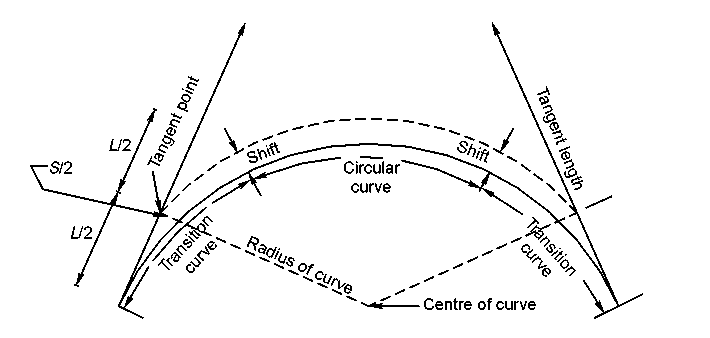
\includegraphics[width=0.7\linewidth]{horizontal_curve_geometry}
    \caption{Annotated geometry of a horizontal curve}
    \label{fig:horizontal-curve-geometry}
\end{figure}

The aim of this section is to work through the method for designing a transition curve. Generally, this will be done using a software programme, but it is always useful to know how this would be done manually.

This will also demonstrate how some of the equations you have already met can be used in designing a track alignment

\subsection*{Worked example}

A metro has the following design parameters:
\begin{itemize}
    \item Velocity $V=$ \qty{80}{km/h}
    \item Radius $R=$ \qty{400}{m}
    \item Max applied cant $E_{a(max)}=$ \qty{150}{mm}
    \item Max cant deficiency $D_{(max)}=$ \qty{90}{mm}
    \item Max cant gradient $CG=$ \num{1} in \num{100}
    \item Max rate of change in cant $\Delta E=$ \qty{55}{mm/s}
\end{itemize}

Calculate:
\begin{itemize}
    \item equilibrium cant $E_q$ (\unit{mm})
    \item applied cant $E_a$ (\unit{mm})
    \item transition length $L_{tr}$ (\unit{m})
    \item curve offset $S_c$ (\unit{m})
    \item $x$ \& $y$ co-ordinate of the transition at \num{4} locations along its length (\unit{m})
\end{itemize}

\subsubsection*{Equilibrium cant}

\begin{equation}
    E_q=\frac{11.82 \cdot V^2}{R}=\frac{11.82 \cdot 80^2}{400} = 189
\end{equation}

$E_q=$ \qty{189}{mm}

\subsubsection*{Applied cant}

Previously, where we used the assumption in equation \ref{eq:e_rot} that applied cant was two thirds of the equilibrium cant, we are now going to use a ratio between the maximum specified applied cant and cant deficiency ($E_{a(max)}$ and $D_{(max)}$) in order to calculate $E_a$ and $D$.

\begin{equation}
    E_a=\frac{E_{a(max)}}{E_{a(max)}+D_{(max)}}E_q = \frac{150}{150+90}E_q = 118
\end{equation}

Rounded to nearest \qty{5}{mm}, $E_a=$ \qty{120}{mm}

\subsubsection*{Cant deficiency}

\begin{equation}
    D=E_q-E_a=189-120=69
\end{equation}

$D=$ \qty{69}{mm}

\subsubsection*{Transition curve length}

This can be derived from either the max cant gradient (equation \ref{eq:ltr_gh}) or the max rate of change in cant (equation \ref{eq:cc}).

\begin{equation}
    \label{eq:ltr_gh}
    L_{tr} = E_a \cdot CG = 120 \cdot 500 = 60
\end{equation}

\begin{equation}
    \label{eq:cc}
    L_{tr} = \frac{E_a \cdot V}{\Delta E \cdot 3.6} = \frac{120 \cdot 80}{55 \cdot 3.6} = 48.5
\end{equation}

The actual transition length we want to design to is the higher result value of these equation, so: $L_{tr}=$ \qty{60}{m} 

\subsubsection*{Curve shift}

This is how far the curve is moved inwards.

\begin{equation}
    S_c=\frac{L_{tr}^2}{24 \cdot R} = \frac{60^2}{24 \cdot 400} = 0.375
\end{equation}

$S_c=$ \qty{0.375}{m}

\begin{figure}[h]
    \centering
    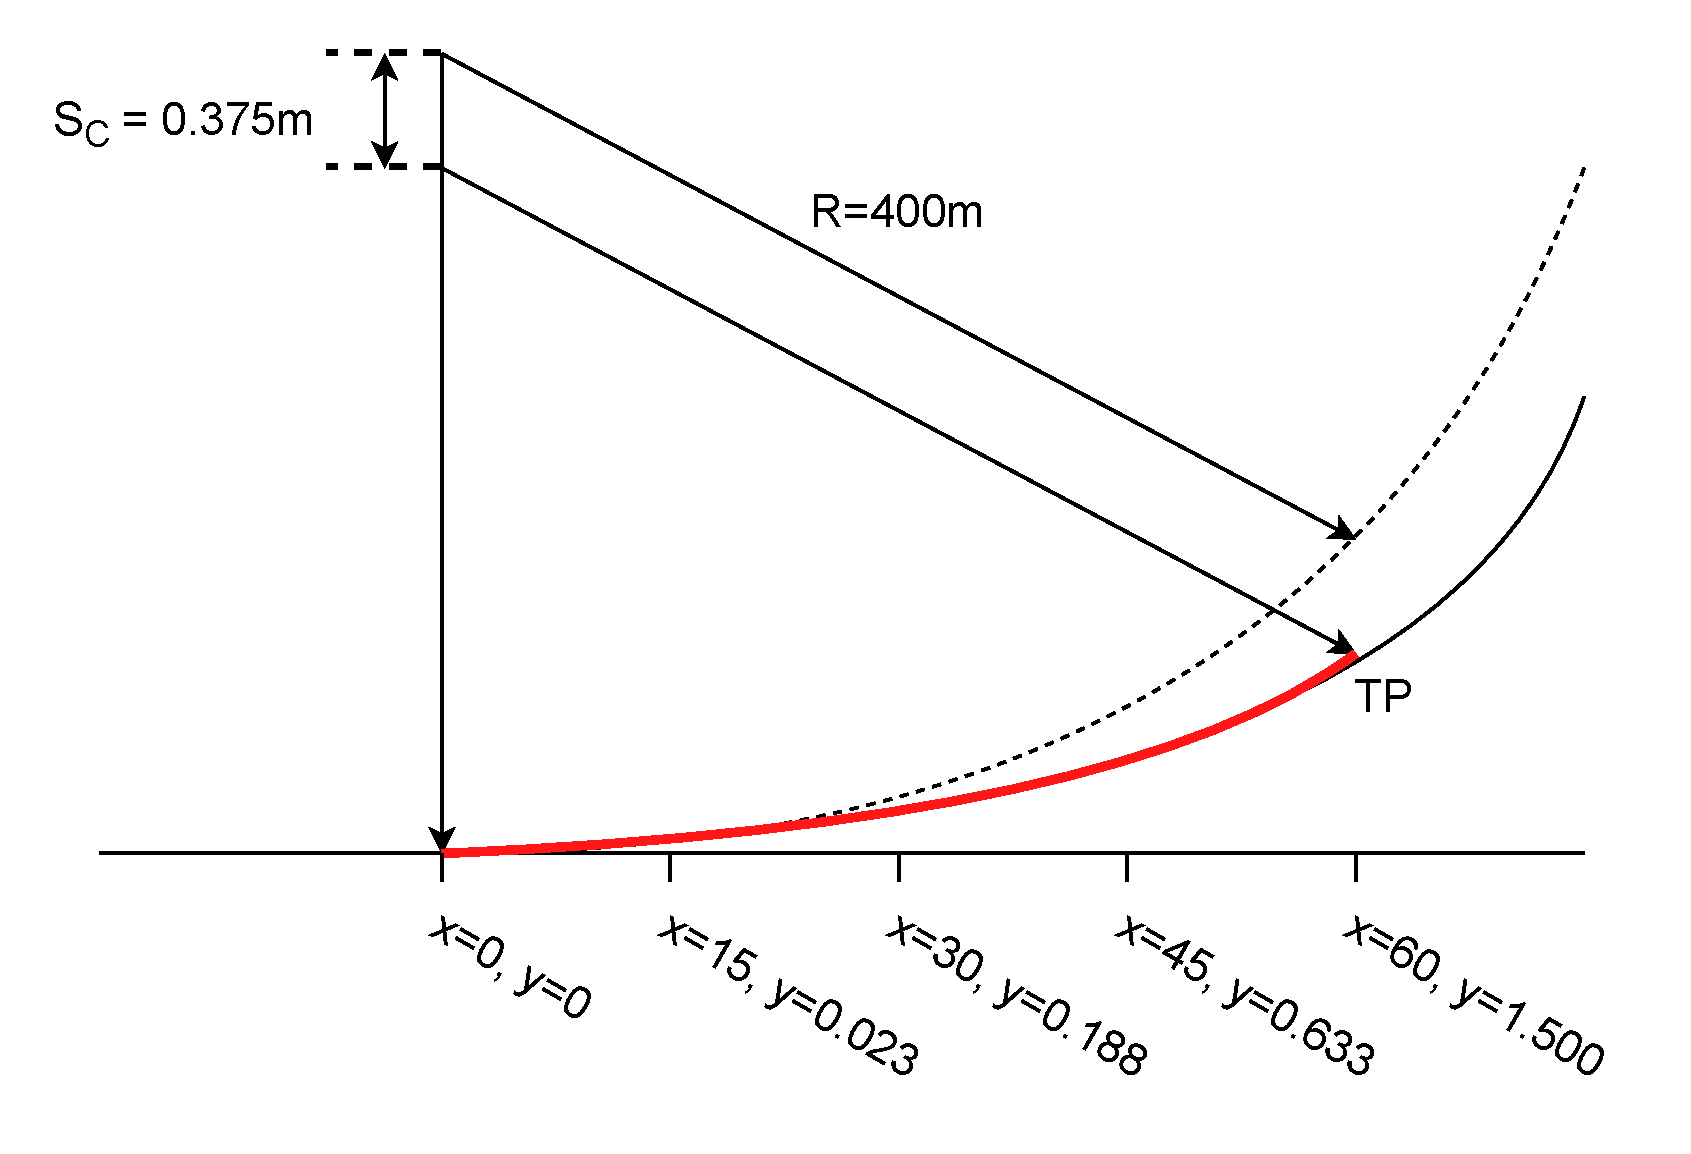
\includegraphics[width=0.9\linewidth]{track-alignment-worksheet-horizontal-curve.drawio}
    \caption{Diagram of horizontal curve worked example}
    \label{fig:hoz-cur-example}
\end{figure}

Figure \ref{fig:hoz-cur-example} shows how the length of the radius is reduced by \qty{0.375}{m} at the start of the transition curve.

\subsubsection*{Curve Co-ordinates}

To calculate the co-ordinates along the transition to a circular curve, the following two equations are used.

\begin{equation}
    x=s
\end{equation}

\begin{equation}
    y=\frac{s^3}{6 \cdot R \cdot L_{tr}}
\end{equation}

The results at 4 co-ordinates along the transition curve are shown in the table below and in figure \ref{fig:hoz-cur-example}.

\begin{table}[h]
\centering
\begin{tabular}{@{}llllll@{}}
\toprule
$x$ & \num{0}     & \num{15}    & \num{30}    & \num{45}    & \num{60}    \\ 
$y$ & \num{0.000} & \num{0.023} & \num{0.188} & \num{0.633} & \num{1.500} \\ \bottomrule
\end{tabular}
\end{table}

\subsection*{Questions}


\begin{questions}
\question 
A railway has the following design parameters:

\begin{itemize}
    \item Velocity $V=$ \qty{160}{km/h}
    \item Radius $R=$ \qty{1250}{m}
    \item Max applied cant $E_{a(max)}=$ \qty{150}{mm}
    \item Max cant deficiency $D_{(max)}=$ \qty{110}{mm}
    \item Max cant gradient $CG=$ \num{1} in \num{400}
    \item Max rate of change in cant $\Delta E=$ \qty{55}{mm/s}
\end{itemize}

Calculate the equilibrium cant, applied cant, transition length, curve offset and the $x$ \& $y$ co-ordinates of the transition at 4 locations along its length.

\begin{solution}
\begin{equation}
    E_q=\frac{11.82 \cdot V^2}{R}=\frac{11.82 \cdot 160^2}{1250} = 242
\end{equation}

$E_q=$ \qty{242}{mm}

\begin{equation}
    E_a=\frac{E_{a(max)}}{E_{a(max)}+D_{(max)}}E_q = \frac{150}{150+110}E_q = 140
\end{equation}

Rounded to nearest \qty{5}{mm}, $E_a=$ \qty{140}{mm}

\begin{equation}
    D=E_q-E_a=242-140=102
\end{equation}

$D=$ \qty{102}{mm}

\begin{equation}
    L_{tr}=E_a \cdot CG = 140 \cdot 400 = 56
\end{equation}

\begin{equation}
    L_{tr} = \frac{E_a \cdot V}{\Delta E \cdot 3.6} = \frac{140 \cdot 160}{55 \cdot 3.6} = 113
\end{equation}

$L_{tr}=$ \qty{113}{m}

\begin{equation}
    S_c=\frac{L_{tr}^2}{24 \cdot R} = \frac{160^2}{24 \cdot 1250} = 0.427
\end{equation}

$S_c=$ \qty{0.375}{m}

\vspace{1cm}

\begin{tabular}{@{}llllll@{}}
\toprule
$x$ & \num{0}     & \num{15}    & \num{30}    & \num{45}    & \num{60}    \\ 
$y$ & \num{0.000} & \num{0.004} & \num{0.032} & \num{0.107} & \num{0.255} \\ \bottomrule
\end{tabular}

\end{solution}

\question 
A railway has the following design parameters:

\begin{itemize}
    \item Velocity $V=$ \qty{120}{km/h}
    \item Radius $R=$ \qty{1050}{m}
    \item Max applied cant $E_{a(max)}=$ \qty{110}{mm}
    \item Max cant deficiency $D_{(max)}=$ \qty{90}{mm}
    \item Max cant gradient $CG=$ \num{1} in \num{450}
    \item Max rate of change in cant $\Delta E=$ \qty{55}{mm/s}
\end{itemize}

Calculate the equilibrium cant, applied cant, transition length, curve offset and the $x$ \& $y$ co-ordinates of the transition at 4 locations along its length.

\begin{solution}
\begin{equation}
    E_q=\frac{11.82 \cdot V^2}{R}=\frac{11.82 \cdot 120^2}{1050} = 162
\end{equation}

$E_q=$ \qty{162}{mm}

\begin{equation}
    E_a=\frac{E_{a(max)}}{E_{a(max)}+D_{(max)}}E_q = \frac{110}{90}E_q = 89
\end{equation}

Rounded to nearest \qty{5}{mm}, $E_a=$ \qty{90}{mm}

\begin{equation}
    D=E_q-E_a=162-90=72
\end{equation}

$D=$ \qty{72}{mm}

\begin{equation}
    L_{tr}=E_a \cdot CG = 90 \cdot 450 = 40.5
\end{equation}

\begin{equation}
    L_{tr} = \frac{E_a \cdot V}{\Delta E \cdot 3.6} = \frac{90 \cdot 120}{55 \cdot 3.6} = 54.5
\end{equation}

$L_{tr}=$ \qty{54.5}{m}

\begin{equation}
    S_c=\frac{L_{tr}^2}{24 \cdot R} = \frac{120^2}{24 \cdot 1050} = 0.118
\end{equation}

$S_c=$ \qty{0.118}{m}

\vspace{1cm}

\begin{tabular}{@{}llllll@{}}
\toprule
$x$ & \num{0}     & \num{15}    & \num{30}    & \num{45}    & \num{60}    \\ 
$y$ & \num{0.000} & \num{0.010} & \num{0.079} & \num{0.265} & \num{0.629} \\ \bottomrule
\end{tabular}

\end{solution}

\question Design a curve for HS2. Highlight any assumptions you have made in order to be able to complete this task. 

\end{questions}

\newpage
\section{Designing Vertical Curves}

A vertical curve is a parabolic curve between two grades on a railway. Its aim is to make the ride smooth.

\begin{table}[h]
\centering
\caption{Vertical acceleration ($a_v$) limits for vertical curves}
\label{tab:vert-acc-limits}
\begin{tabular}{@{}llll@{}}
\toprule
Criteria  & Standard Limit (\unit{\meter \per \second \squared}) & Maximum Limit (\unit{\meter \per \second \squared}) & Exceptional Limit (\unit{\meter \per \second \squared}) \\ \midrule
Freight   & \num{0.10} & \num{0.22} & \num{0.31} \\
Passenger & \num{0.19} & \num{0.22} & \num{0.31} \\ \bottomrule
\end{tabular}
\end{table}

\subsection*{Worked Example}
Calculate the vertical curve between an upward gradient of \qty{1}{\percent} and a downward gradient of \qty{2.5}{\percent} for a passenger service at the standard limit.

\begin{itemize}
    \item Initial height $H_0=$ \qty{-35}{\meter}
    \item Velocity $V=$ \qty{80}{km/h}
    \item Minimum vertical curve radius $R_{(min)}=$ \qty{2500}{m}
\end{itemize}

\subsubsection*{Vertical acceleration}

Using table \ref{tab:vert-acc-limits}:
\begin{itemize}
    \item Vertical acceleration $a_v =$ \qty{0.19}{\meter \per \second \squared}
\end{itemize}

\subsubsection*{Vertical Curve Radius}

First, work out the length of the radius.

\begin{equation}
    R_{vc}=\frac{V^2}{33.1776 \cdot a_v}=\frac{80^2}{33.1776 \cdot 0.19} = 1015
\end{equation}

However, this is below the minimum limit for vertical curve radius, therefore.

$R_{vc}=$ \qty{2500}{m}

\subsubsection*{Curve Length}

Next, work out the longitudinal linear length of the vertical curve.

\begin{itemize}
    \item Initial gradient $G_1=$ \qty{1}{\percent}
    \item Final gradient $G_2=$ \qty{-2.5}{\percent}
\end{itemize}

\begin{equation}
    L_{vc} = \frac{R_{vc}(G_1-G_2)}{100}=\frac{2500(1-(-2.5))}{100}=87.5
\end{equation}

$L_{vc}=$ \qty{87.5}{m}

\begin{figure}[p]
    \centering
    \begin{subfigure}[b]{0.48\textwidth}
        \centering
        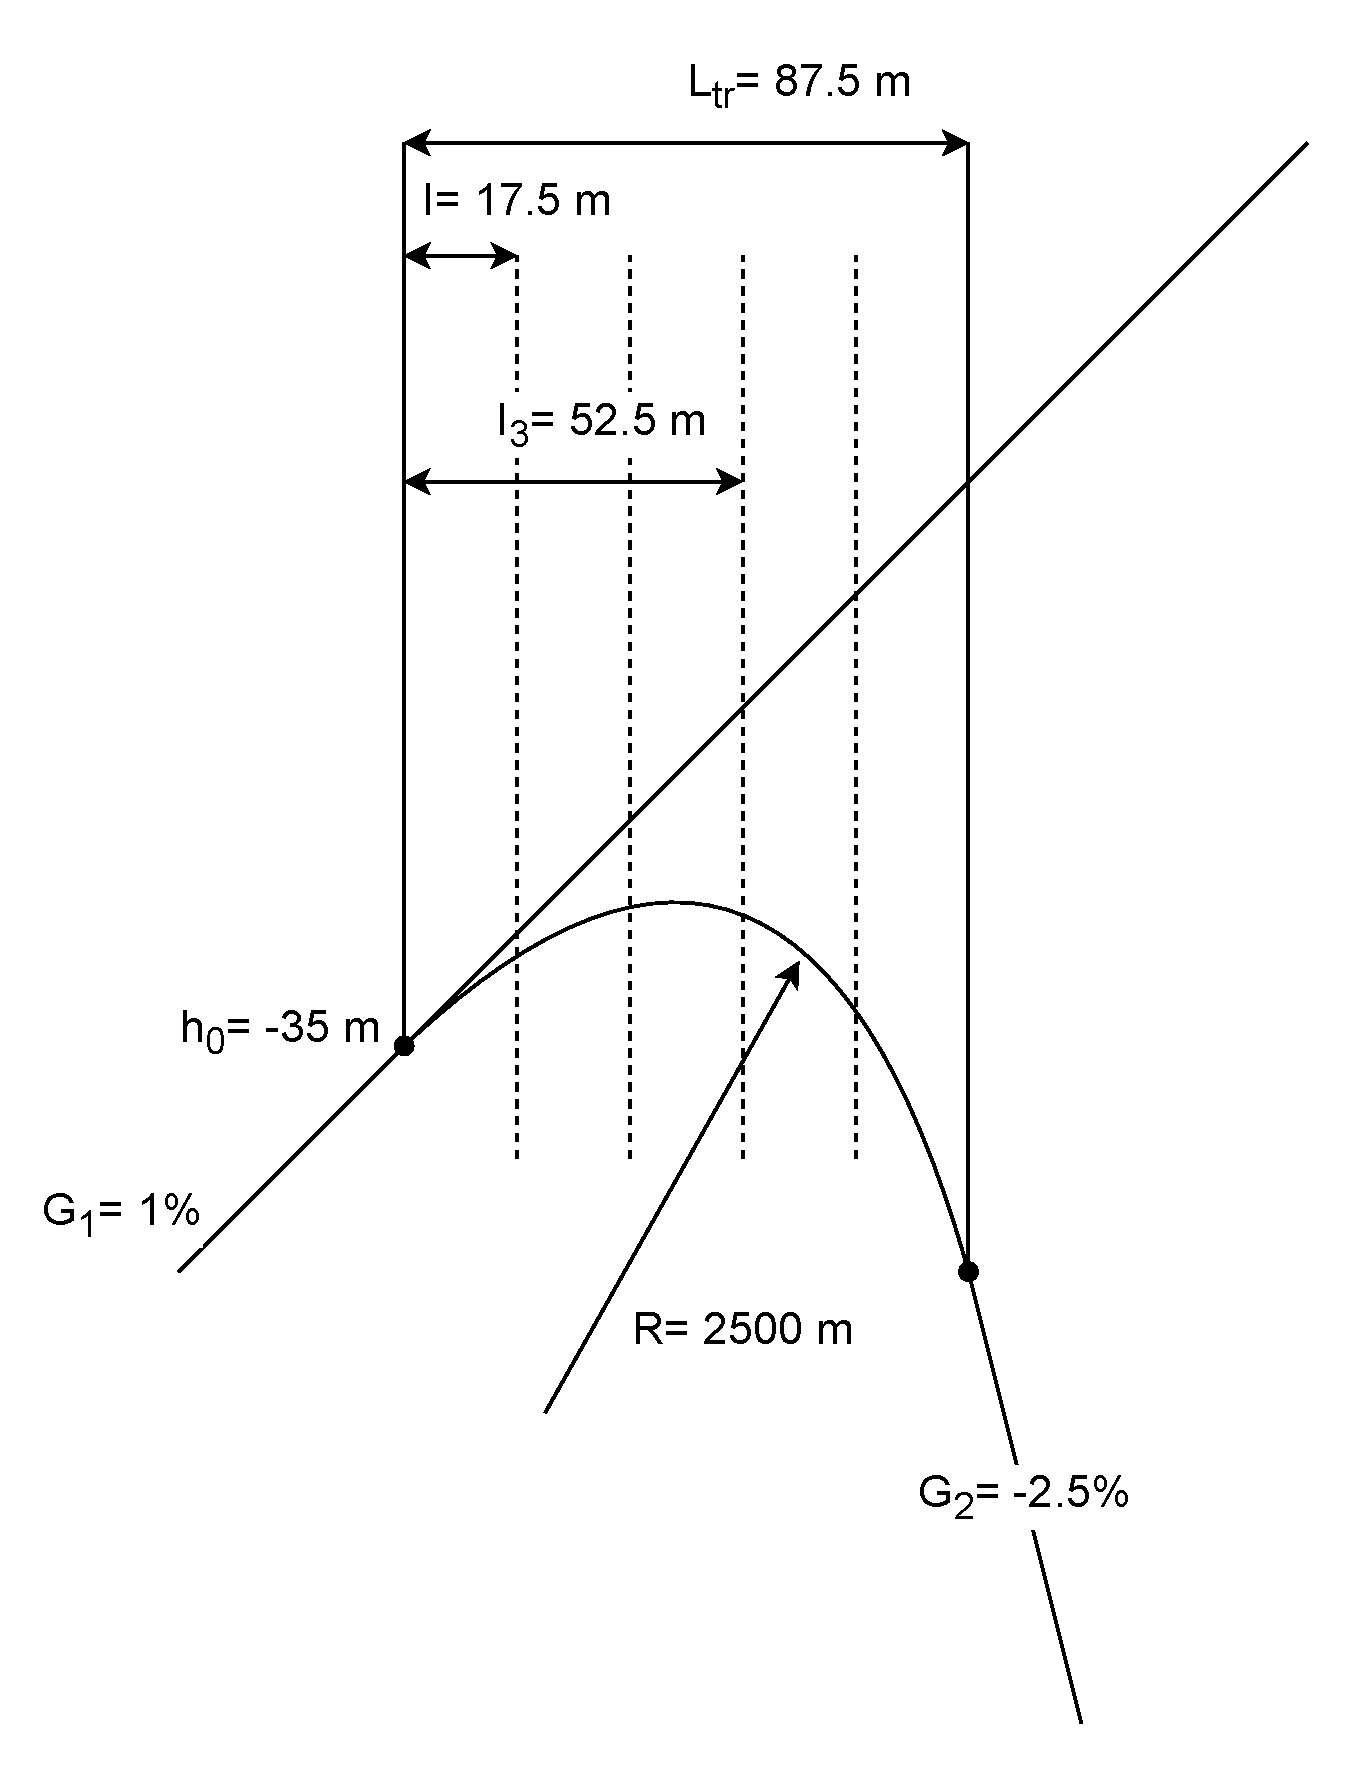
\includegraphics[width=\textwidth]{images/track-alignment-worksheet-vertical-curve-intervals.drawio.pdf}
        \caption{interval}
        \label{fig:vertical-curve-interval}
    \end{subfigure}
    \hfill
    \begin{subfigure}[b]{0.48\textwidth}
        \centering
        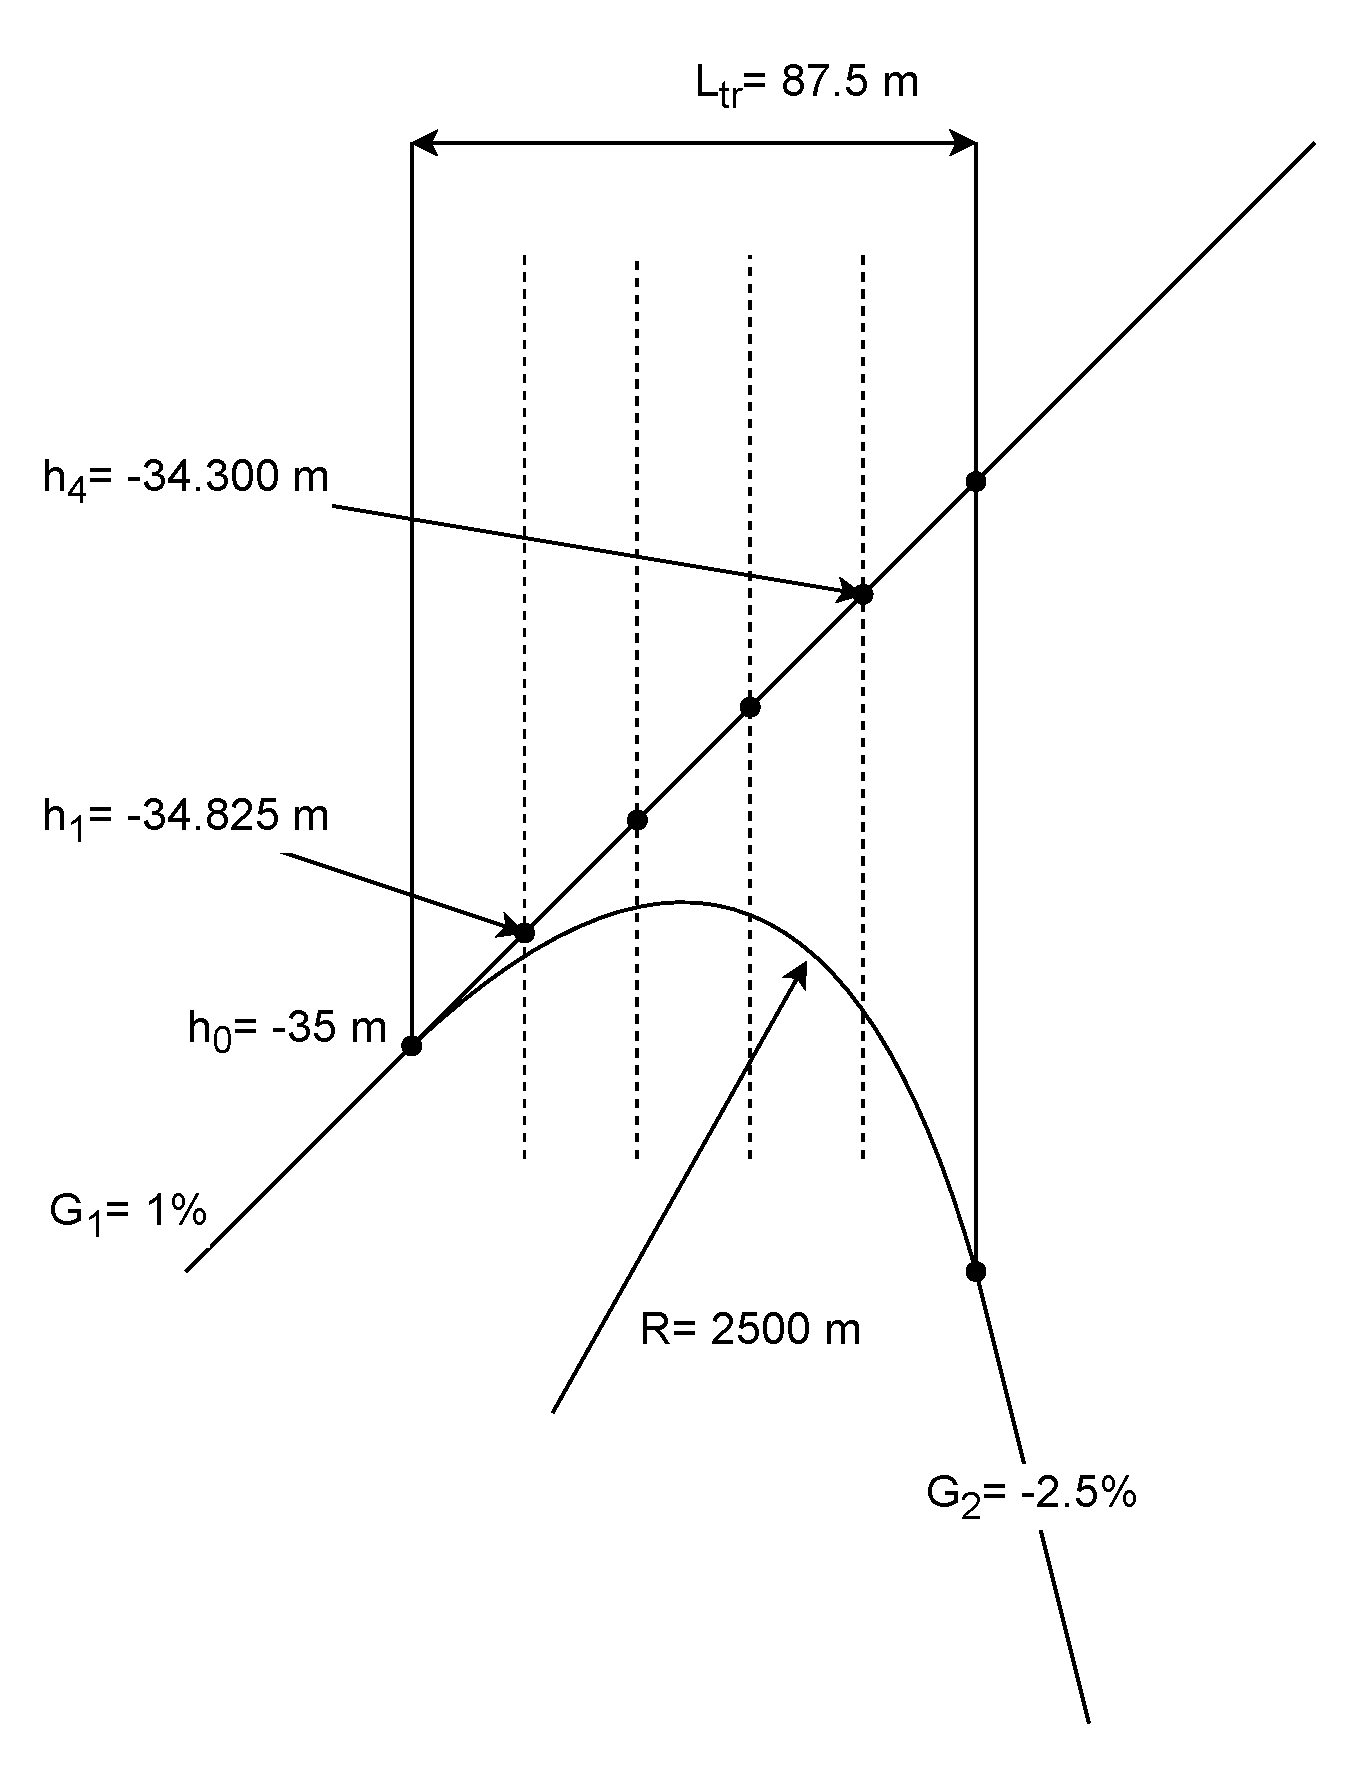
\includegraphics[width=\textwidth]{images/track-alignment-worksheet-vertical-curve-heights.drawio.pdf}
        \caption{grade levels}
        \label{fig:vertical-curve-height}
    \end{subfigure}
    
    \begin{subfigure}[b]{0.48\textwidth}
        \centering
        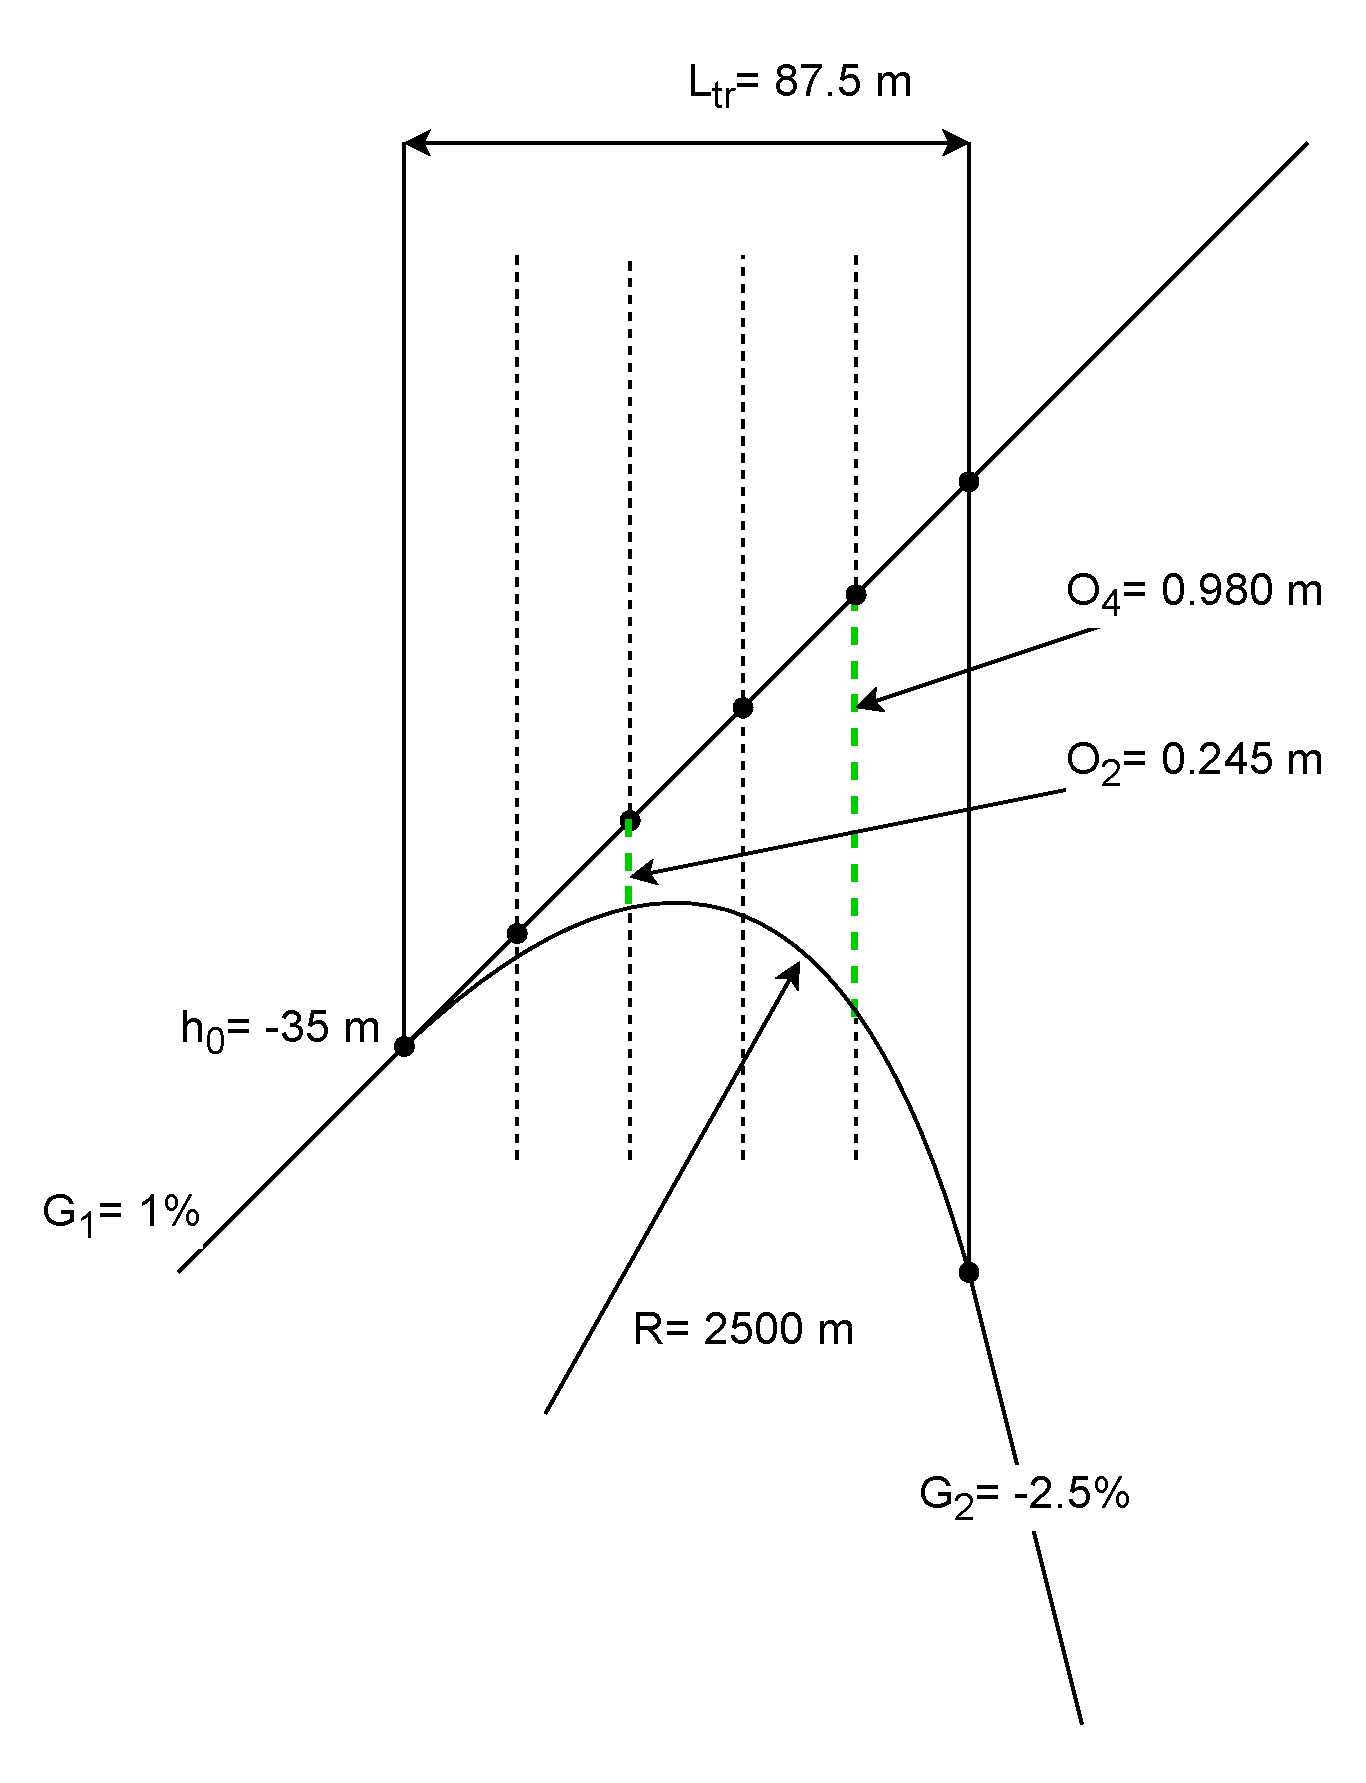
\includegraphics[width=\textwidth]{images/track-alignment-worksheet-vertical-curve-extension.drawio.pdf}
        \caption{extension}
        \label{fig:vertical-curve-extension}
    \end{subfigure}
    \hfill
    \begin{subfigure}[b]{0.48\textwidth}
        \centering
        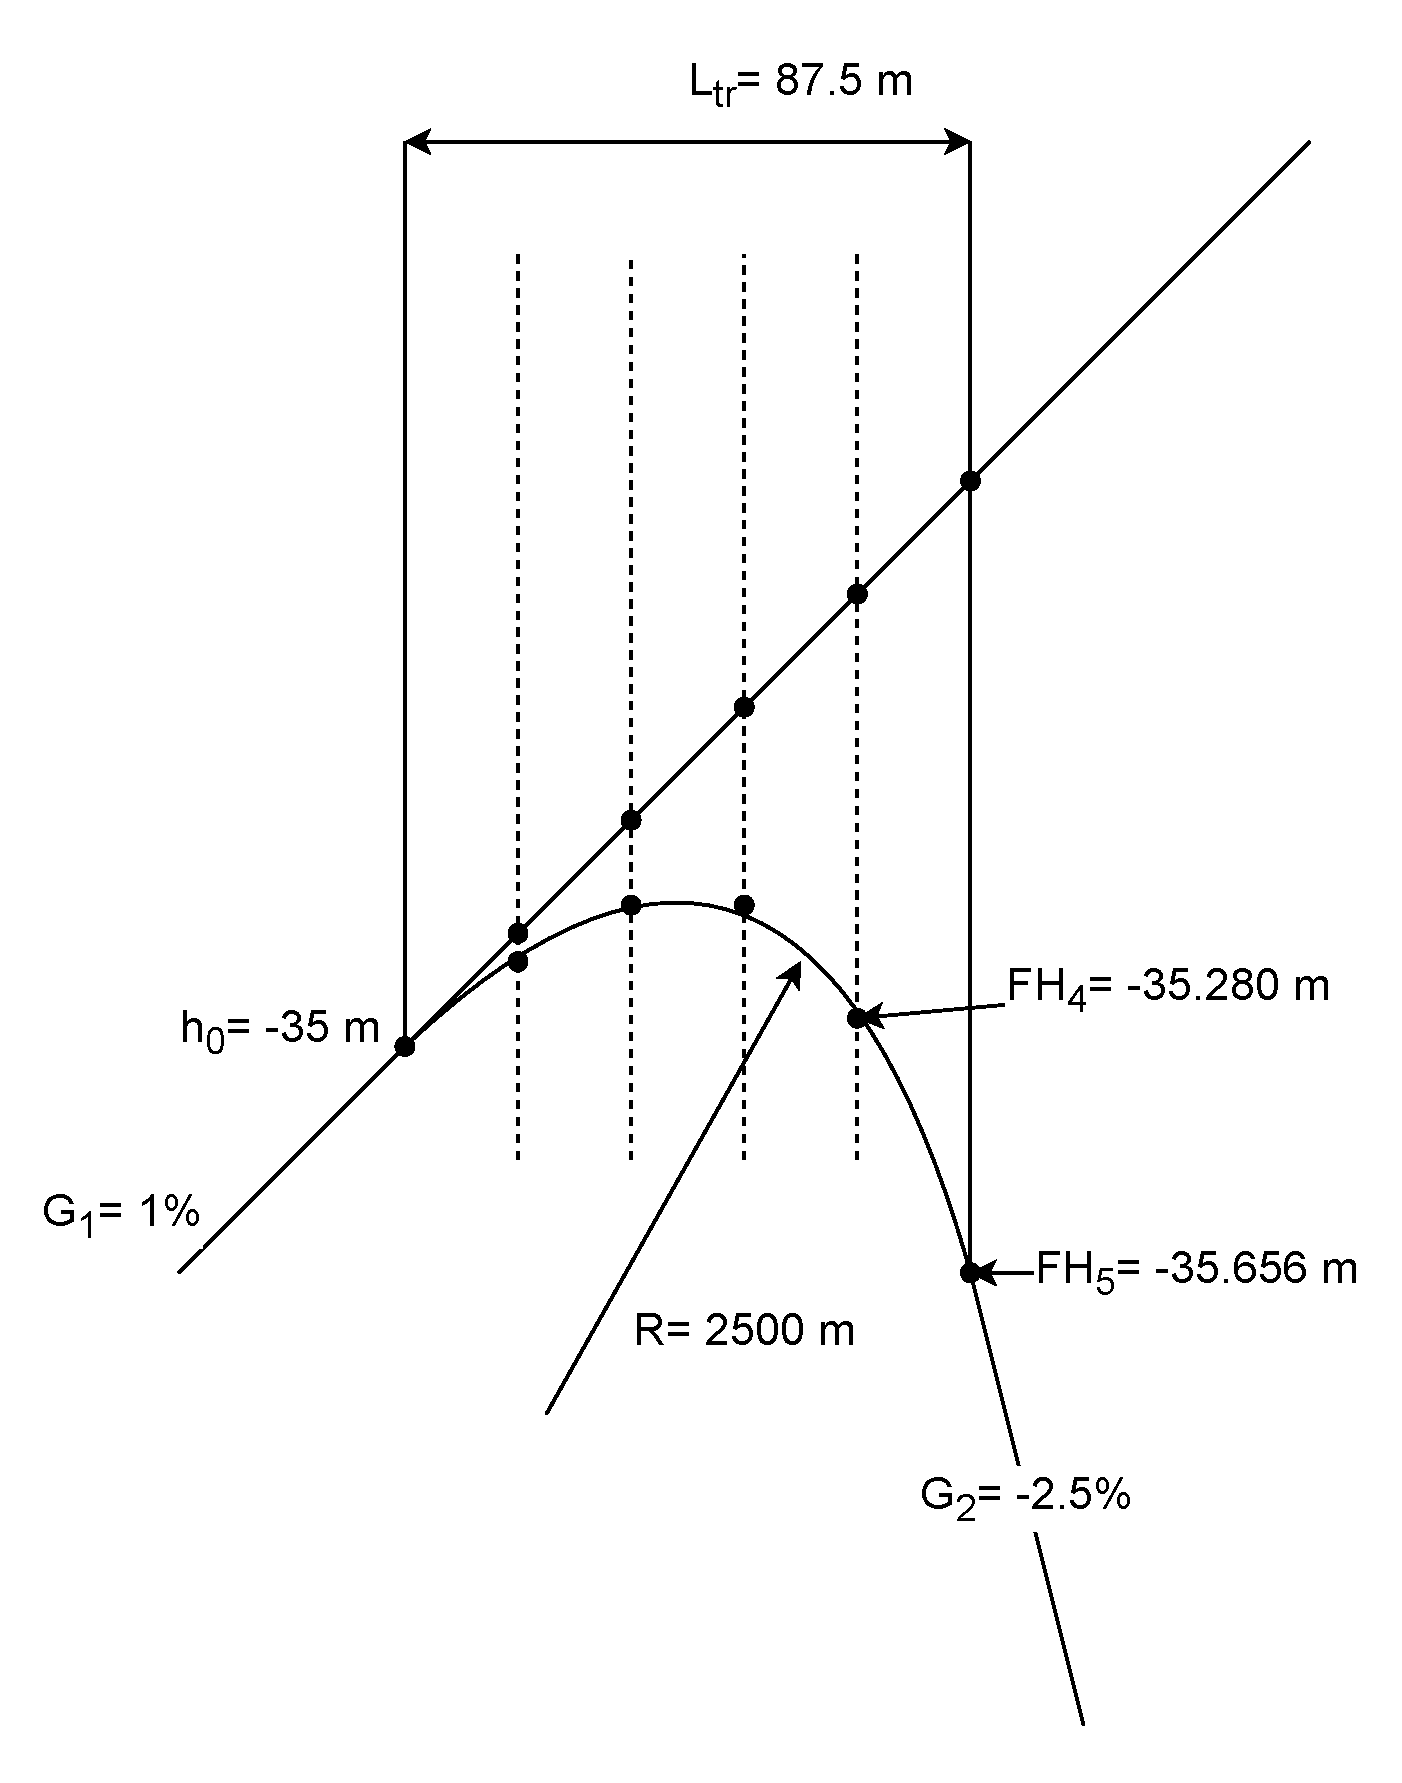
\includegraphics[width=\textwidth]{images/track-alignment-worksheet-vertical-curve-fh.drawio.pdf}
        \caption{final height}
        \label{fig:vertical-curve-fh}
    \end{subfigure}
    \caption{4 Diagrams showing the states of calculating}
    \label{fig:vertical-curve-diagrams}
\end{figure}

\subsubsection*{Intervals}

Next, assume there are 5 intervals and calculate the longitudinal length between each interval, this measure is shown in figure \ref{fig:vertical-curve-interval}.

\begin{itemize}
    \item Number of intervals $N=$ \num{5}
\end{itemize}

\begin{equation}
    I = \frac{L_{vc}}{N} = \frac{87.5}{5} = 17.5
\end{equation}

Next, calculate how far each interval is from the initial transition point at $h_0$.

\begin{equation}
    I_n = I \cdot n
\end{equation}

For the third interval $n=3$

\begin{equation}
    I_3 = 17.5 \cdot 3 = 52.5
\end{equation}

\subsubsection*{Grade level}

Then, calculate the height of each interval point (on the linear project line of the initial gradient), this measure is shown in figure \ref{fig:vertical-curve-height}.

\begin{equation}
    h_n=h_0+\frac{G_1 \cdot I_n}{100}
\end{equation}

for the first interval $n=1$ 

\begin{equation}
    h_1=h_0+\frac{G_1 \cdot I_1}{100}=-35+\frac{1 \cdot 17.5}{100} = -34.825
\end{equation}

\subsubsection*{Extension}

Next, we now have the height of each individual point, so calculate the distance from the interval point to the radial curve, these are the sections shown in green in figure \ref{fig:vertical-curve-extension}.

\begin{equation}
    O_n=\frac{(G_1-G_2) \cdot I_n^2}{200 \cdot L_{vc}}
\end{equation}

for the second interval n=2

\begin{equation}
    O_2=\frac{(G_1-G_2) \cdot I_2^2}{200 \cdot L_{vc}} = \frac{(1-(-2.5)) \cdot 35^2}{200 \cdot 87.5} = 0.245
\end{equation}

\subsubsection*{Final Height}

The final step is therefore to subtract the extension from the grade level at each interval to find the final height, as is shown in figure \ref{fig:vertical-curve-fh}.

\begin{equation}
    FH_n=h_n - O_n
\end{equation}

for the fourth interval n=4

\begin{equation}
    FH_n=h_n - O_n = -34.300-0.980=-35.280
\end{equation}

\subsubsection*{Results Table}

With interval

\begin{table}[h]
\centering
\caption{Worked Example Results Table}
\label{tab:vc_example}
\begin{tabular}{@{}lllll@{}}
\toprule
Interval number & Interval length & Grade level & Extension & Final Height \\
($n$) & $I$ (\unit{m}) & $h$ (\unit{m}) & $O$ (\unit{m}) & $FH$ (\unit{m}) \\
\midrule
\num{0} & \num{0.000}  & \num{-35.000} & \num{0.000} & \num{-35.000} \\
\num{1} & \num{17.500} & \num{-34.825} & \num{0.061} & \num{-34.886} \\
\num{2} & \num{35.000} & \num{-34.650} & \num{0.245} & \num{-34.895} \\
\num{3} & \num{52.500} & \num{-34.475} & \num{0.551} & \num{-35.026} \\
\num{4} & \num{70.000} & \num{-34.300} & \num{0.980} & \num{-35.280} \\
\num{5} & \num{87.500} & \num{-34.125} & \num{1.531} & \num{-35.656} \\ \bottomrule
\end{tabular}
\end{table}

\subsection*{Questions}
\begin{questions}

\question
Calculate the $x$ and $y$ co-ordinates of a vertical curve at \num{5} intervals based on the following parameters for a passenger service with standard limits:
\begin{itemize}
    \item Initial gradient $G_1=$ \qty{2.5}{\percent}
    \item Final gradient $G_2=$ \qty{0}{\percent}
    \item Initial height $H_0=$ \qty{-35}{m}
    \item Velocity $V=$ \qty{80}{km/h}
    \item Minimum vertical curve radius $R_{(min)}=$ \qty{1000}{m}
\end{itemize}

\begin{solution}
Using the standard limit for a passenger service, $a_v=$ \qty{0.19}{\meter \per \second \squared}

\begin{equation}
    R_{vc}=\frac{V^2}{33.1776 \cdot a_v}=\frac{80^2}{33.1776 \cdot 0.19} = 1015
\end{equation}

This is greater than the minimum vertical curve radius so $R_{vc}=$ \qty{1015}.

\begin{equation}
    L_{vc} = \frac{R_{vc}(G_1-G_2)}{100}=\frac{1015(2.5-0)}{100}=25
\end{equation}

$L_{vc}=$ \qty{25}{m}

\begin{equation}
    I = \frac{L_{vc}}{N} = \frac{25}{5} = 5
\end{equation}

\begin{equation}
    I_n = n \cdot I = 5n
\end{equation}

\begin{equation}
    h_n = h_0 + \frac{G_1 \cdot I_n}{100}=-35+\frac{2.5 \cdot 5n}{100}
\end{equation}

\begin{equation}
    O_n = \frac{(G_1-G_2) \cdot I_n^2}{200 \cdot L_{vc}} = \frac{(2.5-0)\cdot (5n)^2}{200 \cdot 25}
\end{equation}

\begin{equation}
    FH_n = h_n - O_n = -35+\frac{2.5 \cdot 5n}{100} - \frac{(2.5-0)\cdot (5n)^2}{200 \cdot 25}
\end{equation}

\vspace{1cm}

\begin{tabular}{@{}lllll@{}}
\toprule
Interval number & Interval length & Grade level & Extension & Final Height \\
($n$) & $I$ (\unit{m}) & $h$ (\unit{m}) & $O$ (\unit{m}) & $FH$ (\unit{m}) \\
\midrule
\num{0} & \num{0}  & \num{-35.000} & \num{0.000} & \num{-35.000} \\
\num{1} & \num{5}  & \num{-34.873} & \num{0.013} & \num{-34.886} \\
\num{2} & \num{10} & \num{-34.746} & \num{0.051} & \num{-34.797} \\
\num{3} & \num{15} & \num{-34.619} & \num{0.114} & \num{-34.733} \\
\num{4} & \num{20} & \num{-34.492} & \num{0.203} & \num{-34.695} \\
\num{5} & \num{25} & \num{-34.365} & \num{0.317} & \num{-35.683} \\ \bottomrule
\end{tabular}

\end{solution}

\question
Calculate the $x$ and $y$ co-ordinates of a vertical curve at \num{5} intervals based on the following parameters for a freight service with standard limits:
\begin{itemize}
    \item Initial gradient $G_1=$ \qty{1.5}{\percent}
    \item Final gradient $G_2=$ \qty{-1}{\percent}
    \item Initial height $H_0=$ \qty{0}{m}
    \item Velocity $V=$ \qty{80}{km/h}
    \item Minimum vertical curve radius $R_{(min)}=$ \qty{2000}{m}
\end{itemize}

\begin{solution}
Using the standard limit for a passenger service, $a_v=$ \qty{0.10}{\meter \per \second \squared}

\begin{equation}
    R_{vc}=\frac{V^2}{33.1776 \cdot a_v}=\frac{80^2}{33.1776 \cdot 0.10} = 1929.012
\end{equation}

This is less than the minimum vertical curve radius so $R_{vc}=$ \qty{2000}.

\begin{equation}
    L_{vc} = \frac{R_{vc}(G_1-G_2)}{100}=\frac{2000(1.5-(-1))}{100}=50
\end{equation}

$L_{vc}=$ \qty{50}{m}

\begin{equation}
    I = \frac{L_{vc}}{N} = \frac{50}{5} = 10
\end{equation}

\begin{equation}
    I_n = n \cdot I = 10n
\end{equation}

\begin{equation}
    h_n = h_0 + \frac{G_1 \cdot I_n}{100}=0+\frac{1.5 \cdot 10n}{100}
\end{equation}

\begin{equation}
    O_n = \frac{(G_1-G_2) \cdot I_n^2}{200 \cdot L_{vc}} = \frac{(1.5-(-1))\cdot (10n)^2}{200 \cdot 50}
\end{equation}

\begin{equation}
    FH_n = h_n - O_n = 0+\frac{1.5 \cdot 10n}{100} - \frac{(1.5-(-1))\cdot (10n)^2}{200 \cdot 50}
\end{equation}

\vspace{1cm}

\begin{tabular}{@{}lllll@{}}
\toprule
Interval number & Interval length & Grade level & Extension & Final Height \\
($n$) & $I$ (\unit{m}) & $h$ (\unit{m}) & $O$ (\unit{m}) & $FH$ (\unit{m}) \\
\midrule
\num{0} & \num{0}  & \num{0.000} & \num{0.000} & \num{0.000} \\
\num{1} & \num{10} & \num{0.150} & \num{0.025} & \num{0.125} \\
\num{2} & \num{20} & \num{0.300} & \num{0.100} & \num{0.200} \\
\num{3} & \num{30} & \num{0.450} & \num{0.225} & \num{0.225} \\
\num{4} & \num{40} & \num{0.600} & \num{0.400} & \num{0.200} \\
\num{5} & \num{50} & \num{0.750} & \num{0.625} & \num{0.125} \\ \bottomrule
\end{tabular}

\end{solution}

\end{questions}

\end{document}
